% Foliensatz: "AFu-Kurs nach DJ4UF" von DK0TU, Amateurfunkgruppe der TU Berlin
% Lizenz: CC BY-NC-SA 3.0 de (http://creativecommons.org/licenses/by-nc-sa/3.0/de/)
% Autoren: Felix Baum DB4UM <baum@campus.tu-berlin.de>
% Überarbeitung: Hendrik Boerma
% Korrekturen: Lars Weiler <dc4lw@darc.de>

\documentclass[aspectratio=169]{beamer}

\usepackage[ngerman]{babel} % deutsche Worttrennung etc.
\usepackage[utf8]{inputenc} % UTF8 Text

\usepackage[super, comma, numbers, square, sort]{natbib}

\usepackage{hyperref}       % Hyperref Package für bessere Referenzen (todo)
\hypersetup{
	colorlinks=false,       %   false: boxed links; true: colored links
    %linkcolor=white,       %   color of internal links (change box color with linkbordercolor)
    citecolor=red,          %   color of links to bibliography
    filecolor=white,        %   color of file links
    urlcolor=blue           %   color of external links
}

\usepackage{multirow}
\usepackage{wasysym}  % Math Symbols like \permil
%\usepackage{colortbl}
%\usepackage{subscript}
%\usepackage{caption}
%\usepackage{setspace}
%\usepackage{xcolor}        % benutze CodeListe

% Footnote
%\usepackage{hanging}
%
%\setbeamertemplate{footnote}{%
%  \hangpara{2em}{1}%
%  \makebox[2em][l]{\insertfootnotemark}\footnotesize\insertfootnotetext\par%
%}


%\usepackage{pgf}
%\usepackage{tikz}
%\usetikzlibrary{arrows,automata}
%\usetikzlibrary{positioning}
%
%\tikzset{
%    state/.style={
%           rectangle,
%           rounded corners,
%           draw=black, very thick,
%           minimum height=2em,
%           minimum width=2pt,
%           inner sep=2pt,
%           text centered,
%           },
%}

%\usepackage{listings}
%\lstset{basicstyle=\small, numberstyle=\tiny, extendedchars=true, numbers=left, numbersep=5pt}
%\lstset{showtabs=false, showspaces=false, showstringspaces=false}
%%\lstset{backgroundcolor=\color{white!75!lightgray}, , frame=single}
%%\lstset{backgroundcolor=\color{white}}
%%\lstset{backgroundcolor=none}
%\lstset{keywordstyle=\color{blue!50!gray},  identifierstyle=\color{black}}
%\lstset{commentstyle=\color{green!50!gray}, stringstyle=\color{red!50!gray}}
%\lstset{language=C, fontadjust=true, tabsize=2, breaklines=true}
%\lstset{backgroundcolor=\color{white!75!lightgray}, caption=\lstname, frame=single}
%\lstset{emphstyle=\color{black}\fbox}
%
%% Keine "Listing:"-Caption
%\captionsetup{labelformat=empty,labelsep=none}
%
%% für mathematische Umgebungen
%\usepackage{amsmath,amsfonts,amssymb}
%
%\lstdefinestyle{Bash}{
%language=Bash,
%frame=single,
%rulecolor=\color{black},
%backgroundcolor=\color{gray!50},
%keywordstyle=\color{black},
%identifierstyle=,
%commentstyle=\color{black},
%stringstyle=\color{magenta!65!white},
%showstringspaces=false,
%basicstyle=\footnotesize\ttfamily\color{black},
%numbers=none,
%breaklines=true,
%captionpos=b
%}

%\usepackage{listings}
%
%\lstdefinestyle{basic}{
%    captionpos=t,%
%    basicstyle=\footnotesize\ttfamily,%
%    numberstyle=\tiny,%
%    numbers=left,%
%    stepnumber=1,%
%    frame=single,%
%    showspaces=false,%
%    showstringspaces=false,%
%    showtabs=false,%
%    %
%    keywordstyle=\color{blue},%
%    identifierstyle=,%
%    commentstyle=\color{gray},%
%    stringstyle=\color{magenta}%
%}



% fließende Boxen haben keinen Abstand
%\fboxsep0mm

% inkludiere Creative Commons Helper
%%%%%%%%%%%%%%%%%%%%%%%%%%%%%%%%%%%%%%%%%%%%%%%%%%%%%%%%%%%%%%%%
%% ccBeamer 0.1, 2007-07-02                                   %%
%% Written by Sebastian Pipping <webmaster@hartwork.org>      %%
%% ---------------------------------------------------------- %%
%% Licensed under Creative Commons Attribution-ShareAlike 3.0 %%
%% http://creativecommons.org/licenses/by-sa/3.0/             %%
%%%%%%%%%%%%%%%%%%%%%%%%%%%%%%%%%%%%%%%%%%%%%%%%%%%%%%%%%%%%%%%%


%% Images
\newcommand{\CcImageBy}[1]{%
	
\includegraphics[scale=#1]{texdata/creative_commons/cc_by_30.pdf}%
}
\newcommand{\CcImageCc}[1]{%
	
\includegraphics[scale=#1]{texdata/creative_commons/cc_cc_30.pdf}%
}
\newcommand{\CcImageDevNations}[1]{%
	
\includegraphics[scale=#1]{texdata/creative_commons/cc_dev_nations_30.pdf}%
}
\newcommand{\CcImageNc}[1]{%
	
\includegraphics[scale=#1]{texdata/creative_commons/cc_nc_30.pdf}%
}
\newcommand{\CcImageNd}[1]{%
	
\includegraphics[scale=#1]{texdata/creative_commons/cc_nd_30.pdf}%
}
\newcommand{\CcImagePd}[1]{%
	
\includegraphics[scale=#1]{texdata/creative_commons/cc_pd_30.pdf}%
}
\newcommand{\CcImageSa}[1]{%
	
\includegraphics[scale=#1]{texdata/creative_commons/cc_sa_30.pdf}%
}
\newcommand{\CcImageSampling}[1]{%
	
\includegraphics[scale=#1]{texdata/creative_commons/cc_sampling_30.pdf}%
}
\newcommand{\CcImageSamplingPlus}[1]{%
	
\includegraphics[scale=#1]{texdata/creative_commons/cc_sampling_plus_30.pdf}%
}


%% Groups
\newcommand{\CcGroupBy}[2]{% zoom, gap
	\CcImageCc{#1}\hspace*{#2}\CcImageBy{#1}%
}
\newcommand{\CcGroupByNc}[2]{% zoom, gap
	\CcImageCc{#1}\hspace*{#2}\CcImageBy{#1}\hspace*{#2}\CcImageNc{#1}%
}
\newcommand{\CcGroupByNcNd}[2]{% zoom, gap
	\CcImageCc{#1}\hspace*{#2}\CcImageBy{#1}\hspace*{#2}\CcImageNc{#1}\hspace*{#2}\CcImageNd{#1}%
}
\newcommand{\CcGroupByNcSa}[2]{% zoom, gap
	\CcImageCc{#1}\hspace*{#2}\CcImageBy{#1}\hspace*{#2}\CcImageNc{#1}\hspace*{#2}\CcImageSa{#1}%
}
\newcommand{\CcGroupByNd}[2]{% zoom, gap
	\CcImageCc{#1}\hspace*{#2}\CcImageBy{#1}\hspace*{#2}\CcImageNd{#1}%
}
\newcommand{\CcGroupBySa}[2]{% zoom, gap
	\CcImageCc{#1}\hspace*{#2}\CcImageBy{#1}\hspace*{#2}\CcImageSa{#1}%
}
\newcommand{\CcGroupDevNations}[2]{% zoom, gap
	\CcImageCc{#1}\hspace*{#2}\CcImageDevNations{#1}%
}
\newcommand{\CcGroupNcSampling}[2]{% zoom, gap
	\CcImageCc{#1}\hspace*{#2}\CcImageNc{#1}\hspace*{#2}\CcImageSampling{#1}%
}
\newcommand{\CcGroupPd}[1]{% zoom
	\CcImagePd{#1}%
}
\newcommand{\CcGroupSampling}[1]{% zoom
	\CcImageSampling{#1}%
}
\newcommand{\CcGroupSamplingPlus}[1]{% zoom
	\CcImageSamplingPlus{#1}%
}


%% Text
\newcommand{\CcLongnameBy}{Attribution}
\newcommand{\CcLongnameByNc}{Attribution-NonCommercial}
\newcommand{\CcLongnameByNcNd}{Attribution-NoDerivs}
\newcommand{\CcLongnameByNcSa}{Attribution-NonCommercial-ShareAlike}
\newcommand{\CcLongnameByNd}{Attribution-NoDerivs}
\newcommand{\CcLongnameBySa}{Attribution-ShareAlike}

\newcommand{\CcNote}[1]{% longname
	This work is licensed under the \textit{Creative Commons #1 3.0 License}.%
}


% generelles Thema auswählen
\usetheme{Goettingen} %Berlin spart ohne Sidebar allerdings angenehm Platz
% AnnArbor | Antibes | Bergen | Berkeley | Berlin | Boadilla | boxes | CambridgeUS | Copenhagen | Darmstadt | default | Dresden | Frankfurt | Goettingen | Hannover | Ilmenau | JuanLesPins | Luebeck | Madrid | Malmoe | Marburg | Montpellier | PaloAlto | Pittsburgh | Rochester | Singapore | Szeged | Warsaw

% Farben wählen
\usecolortheme{beetle}
% beaver | beetle | crane | default | dolphin | dove | fly | lily | orchid | rose | seagull | seahorse | sidebartab | structure | whale | wolverine

% Setze alle Farben auf Grau und Weiß
%\definecolor{craneorange}{RGB}{64,64,64}
%\definecolor{craneblue}{RGB}{255,255,255}

% Schriftart wählen
\usefonttheme{default}
% default | professionalfonts | serif | structurebold | structureitalicserif | structuresmallcapsserif

% Innere Themen(Kopf-, Fuß-, Sidebar usw)
%\useinnertheme{default}
\useinnertheme{circles}
% default | inmargin | rectangles | rounded | circles

% Äußere Themen (Anordnung der inneren, grenzen der Folien etc.)
\useoutertheme{infolines}
% default | infolines | miniframes | shadow | sidebar | smoothbars | smoothtree | split | tree

% Deaktiviere Navigations-Symbole ({} -> leer)
\setbeamertemplate{navigation symbols}{}
%\setbeamertemplate{navigation symbols}{\large \ifnum \insertframenumber <10 0\fi\insertframenumber/\inserttotalframenumber\vspace*{0.2ex}}

% Zeige ein Hintergrundbild
\setbeamertemplate{background canvas}{
        \hspace*{-2.0cm}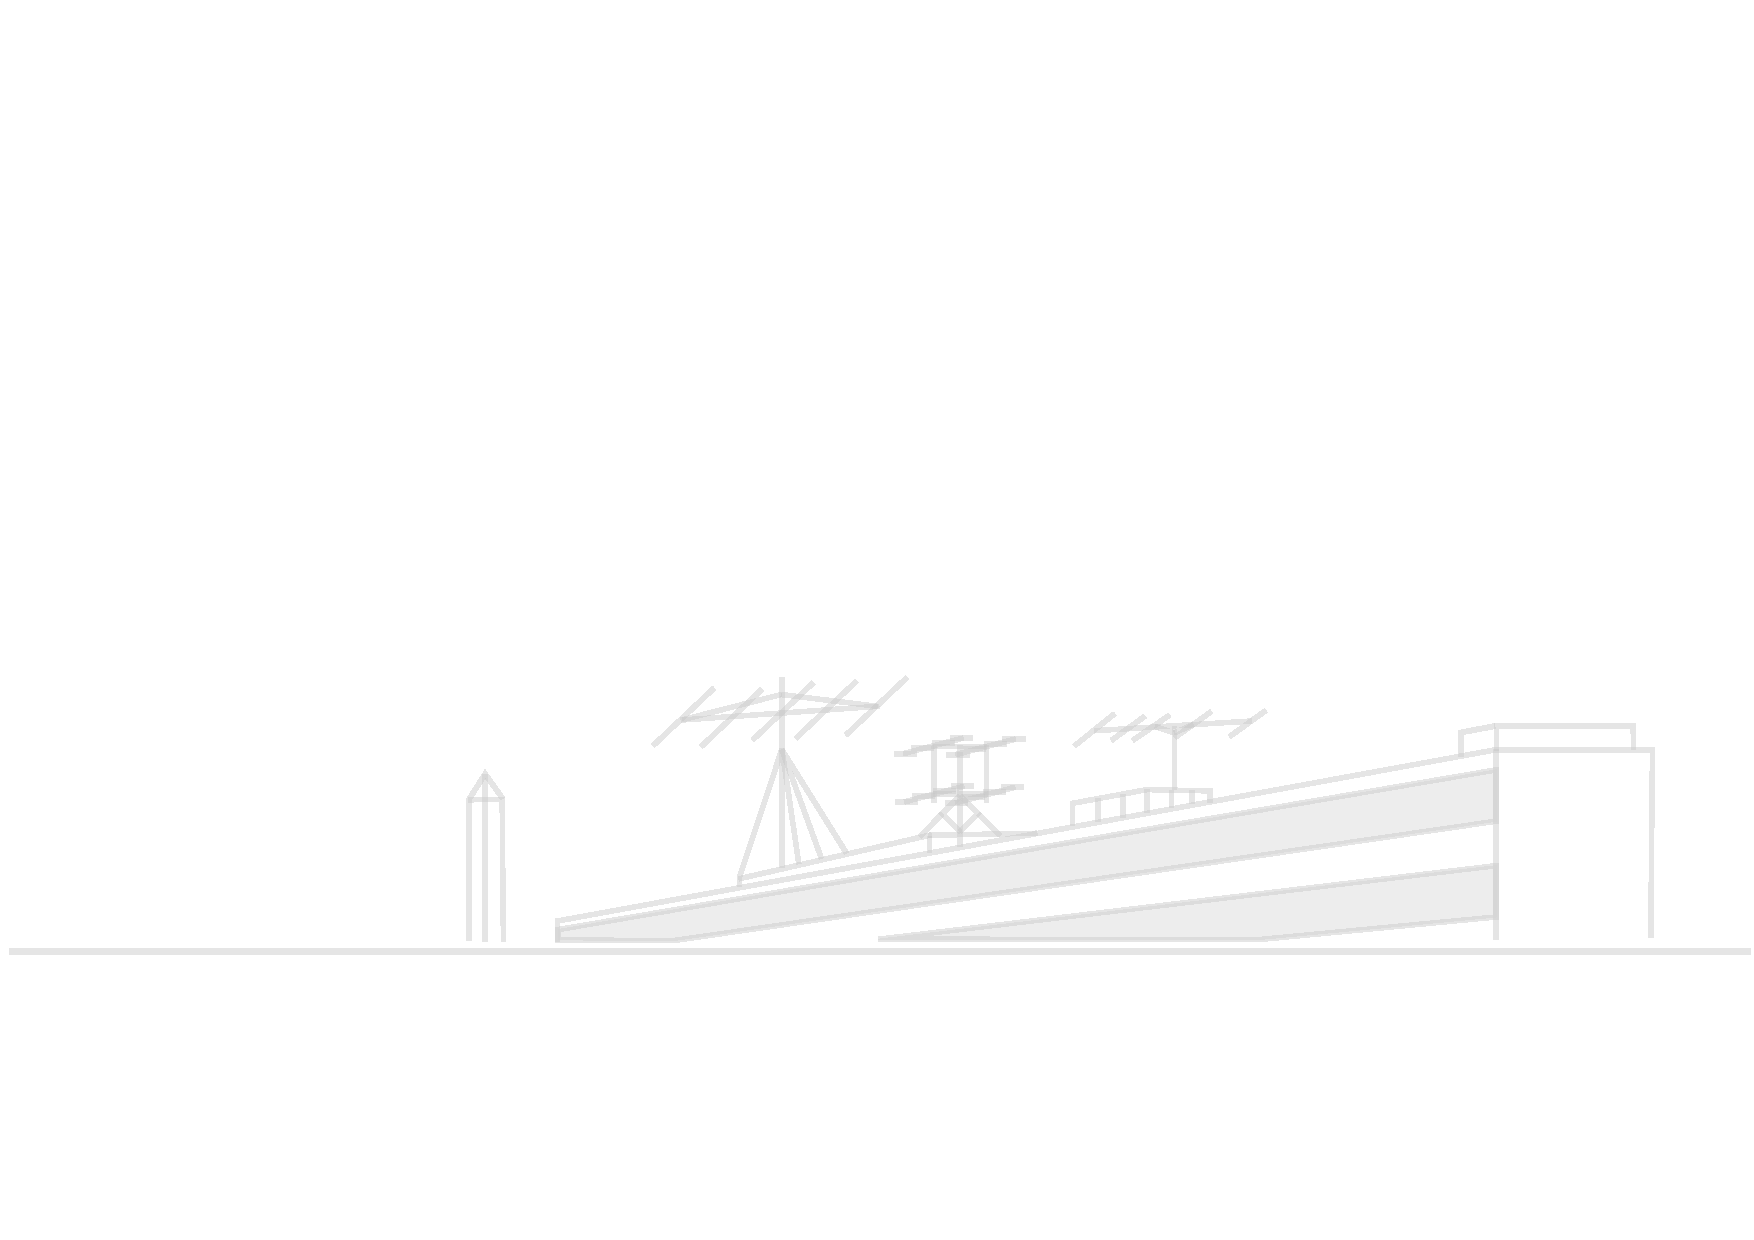
\includegraphics[width=17.8cm]{texdata/dk0tu_rooftop_background.pdf}
}

% Foliennummer einfügen
\setbeamertemplate{footline}[frame number]
%\setbeamertemplate{footline}{}

% Ändere das Zeichen vor jedem item
%\setbeamertemplate{itemize item}{\color{craneorange}$\blacktriangleright$}
%\setbeamertemplate{itemize subitem}{\color{craneorange}$\triangleright$}
%\setbeamertemplate{itemize subsubitem}{\color{craneorange}$\blacktriangleright$}

% Ändert die Blöcke 
\setbeamertemplate{blocks}[rounded][shadow=true]
% default | rounded [shadow=true|false]

%
% Eigene Kommandos
%

% Hack to get natbib and beamer working together. "The beamer user guide suggests
% that only the manual bibliography entry approach is supported"
% on some system it works out of the box, sometimes you need the hack :-(
% so check it --dl7bst
\ifdefined\newblock
    \relax
\else
    \newcommand{\newblock}{}
\fi

% \includedia command to generate png out of a dia file
% NEEDS installed dia and pdflatex option --shell-escape
\newcommand{\includedia}[1]{
    \immediate\write18{/usr/bin/dia #1.dia -e #1_diatmp.png -t png}
}

% RICHIG GROSSER FONT!
\newfont{\bigfont}{cmr10 at 144pt}
\newfont{\smallfont}{cmr10 at 8pt}

% Römische Ziffern
\makeatletter
\newcommand{\rmnum}[1]{\romannumeral #1}
\newcommand{\Rmnum}[1]{\expandafter\@slowromancap\romannumeral #1@}
\makeatother

% Schwarze Überschrift
%\setbeamercolor{frametitle}{fg=black}
%\setbeamercolor{title}{fg=black}

% Item- und Box-Farben
\definecolor{deepBlue}{HTML}{000066}
\setbeamercolor{itemize item}{fg=deepBlue}
\setbeamercolor{itemize subitem}{fg=deepBlue}
\setbeamercolor{description item}{fg=deepBlue}
\setbeamercolor{block title}{fg=deepBlue!100, bg=blue!15}
\setbeamercolor{block body}{fg=black, bg=blue!5}
\setbeamercolor{block title alerted}{fg=deepBlue, bg=red!75}
\setbeamercolor{block body alerted}{fg=black, bg=red!15}
\setbeamercolor*{block title example}{fg=blue!50, bg=blue!10}
\setbeamercolor*{block body example}{fg= blue, bg=blue!5}

%\setbeamercolor{section in head/foot}{parent=palette primary}
%\setbeamercolor{subsection in head/foot}{parent=palette secondary}
%\setbeamercolor{sidebar}{fg=darkblue,bg=yellow!90!orange}
%\setbeamercolor{title in sidebar}{fg=darkblue}
%\setbeamercolor{author in sidebar}{fg=darkblue}
%\setbeamercolor{section in sidebar}{fg=darkblue!10!black}
%\setbeamercolor{subsection in sidebar}{fg=darkblue!50!black}

% Titlepage Infos
\title{AFu-Kurs nach DJ4UF}
\author[DKØTU]{DKØTU\\ \footnotesize{Amateurfunkgruppe der TU Berlin}}
\institute[DKØTU]{\url{http://www.dk0tu.de} }

% PDF-Eigenschaften
\subject{DK0TU-Amateurfunkkurs nach DJ4UF}
\keywords{Amateurfunk Kurs HAM Radio Course CC-BY-NC-SA OpenSource TU Berlin DK0TU}

\subtitle{Technik 02: \\
          Spannung und Strom, Wechselspannung \\[2em]}
\date{Stand 10.10.2016}
 \begin{document}

\begin{frame}
    \titlepage
    \vfill
    \begin{center}
        \ccbyncsaeu\\
        {\tiny This work is licensed under the \em{Creative Commons Attribution-NonCommercial-ShareAlike 3.0 License}.}\\[0.5ex]
         \tiny Amateurfunkgruppe der Technische Universität Berlin (AfuTUB), DKØTU
         %\includegraphics[scale=0.5]{img/DK0TU_Logo.pdf}
    \end{center}
\end{frame}


\section*{Einleitung}

\begin{frame}
  \frametitle{Strom -- Spannung}
  \begin{itemize}
    \item Was ist Spannung/Strom (elektrische)?
    \item Woher bekommt man Spannung/Strom?
  \end{itemize}
\end{frame}

\begin{frame}
  \frametitle{Spannung}
  \begin{center}
    \begin{figure}
      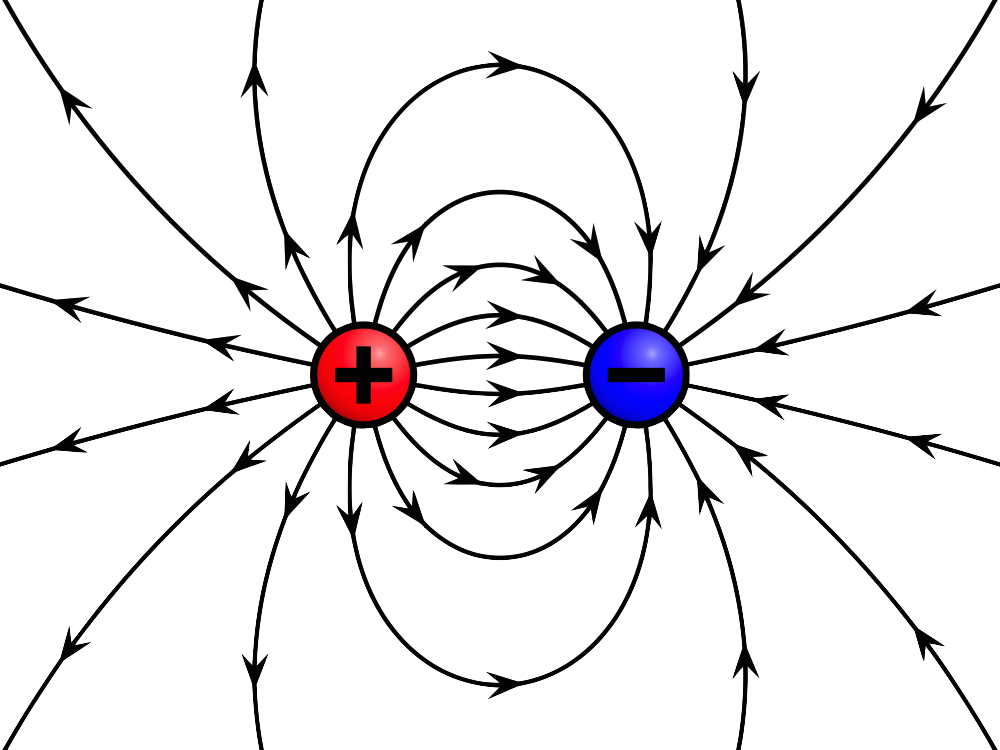
\includegraphics[width=.6\textwidth,height=.75\textheight,keepaspectratio]{e02/ladung.png}
      \attribcaption{Elektrische Spannung wird erzeugt durch die Trennung von Ladungen}{Geek3}{https://commons.wikimedia.org/wiki/File:VFPt_charges_plus_minus_thumb.svg}{\ccbysa}
    \end{figure}
  \end{center}
\end{frame}


\section*{Spannung}

\begin{frame}
  \frametitle{Spannung}
  \begin{center}
    Elektrische Spannung $U$ wird in [$V$] Volt angegeben
  \end{center}
\end{frame}

\begin{frame}
  \frametitle{Batterie}
  \begin{center}
    \begin{figure}
      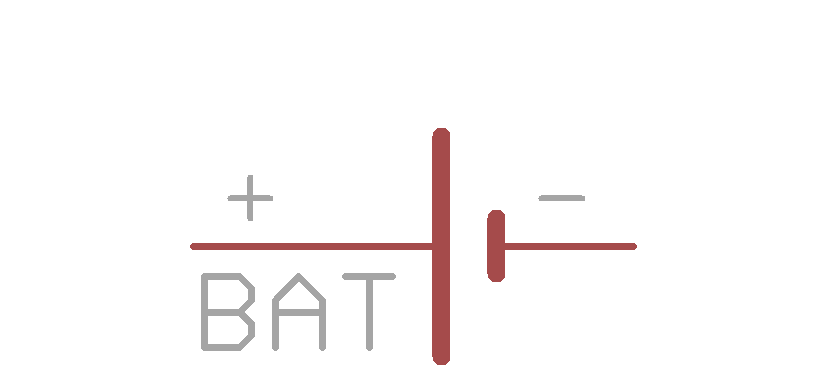
\includegraphics[width=\textwidth,height=.5\textheight,keepaspectratio]{e02/batterieEagle.png}
      \caption{Schaltungszeichen einer Batterie / Batteriezelle}
    \end{figure}
  \end{center}
\end{frame}

\begin{frame}
  \frametitle{9V Batterie}
  \begin{center}
    \begin{figure}
      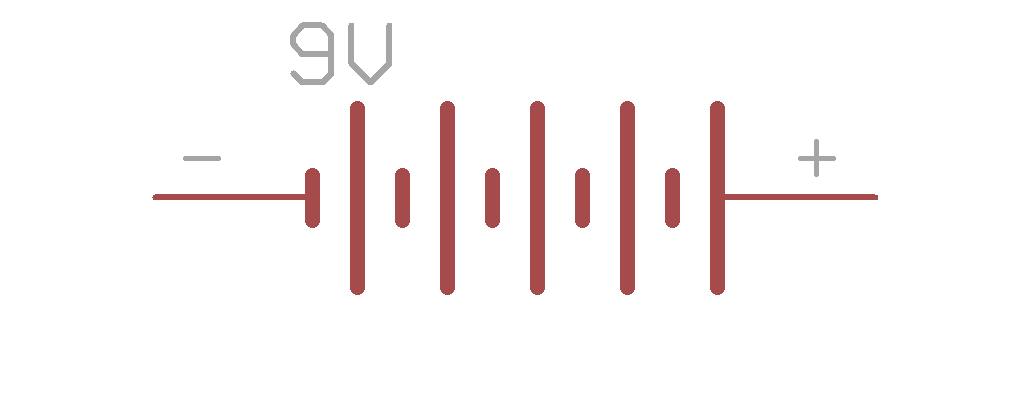
\includegraphics[width=\textwidth,height=.5\textheight,keepaspectratio]{e02/9vBatEagle.png}
      \caption{Schaltungszeichen einer 9V Batterie. Pro Zelle $1,8V$. Werden bei Reihenschaltung addiert.}
    \end{figure}
  \end{center}
\end{frame}

\begin{frame}
  \frametitle{Spannung bestimmen}
  \begin{center}
    \begin{figure}
      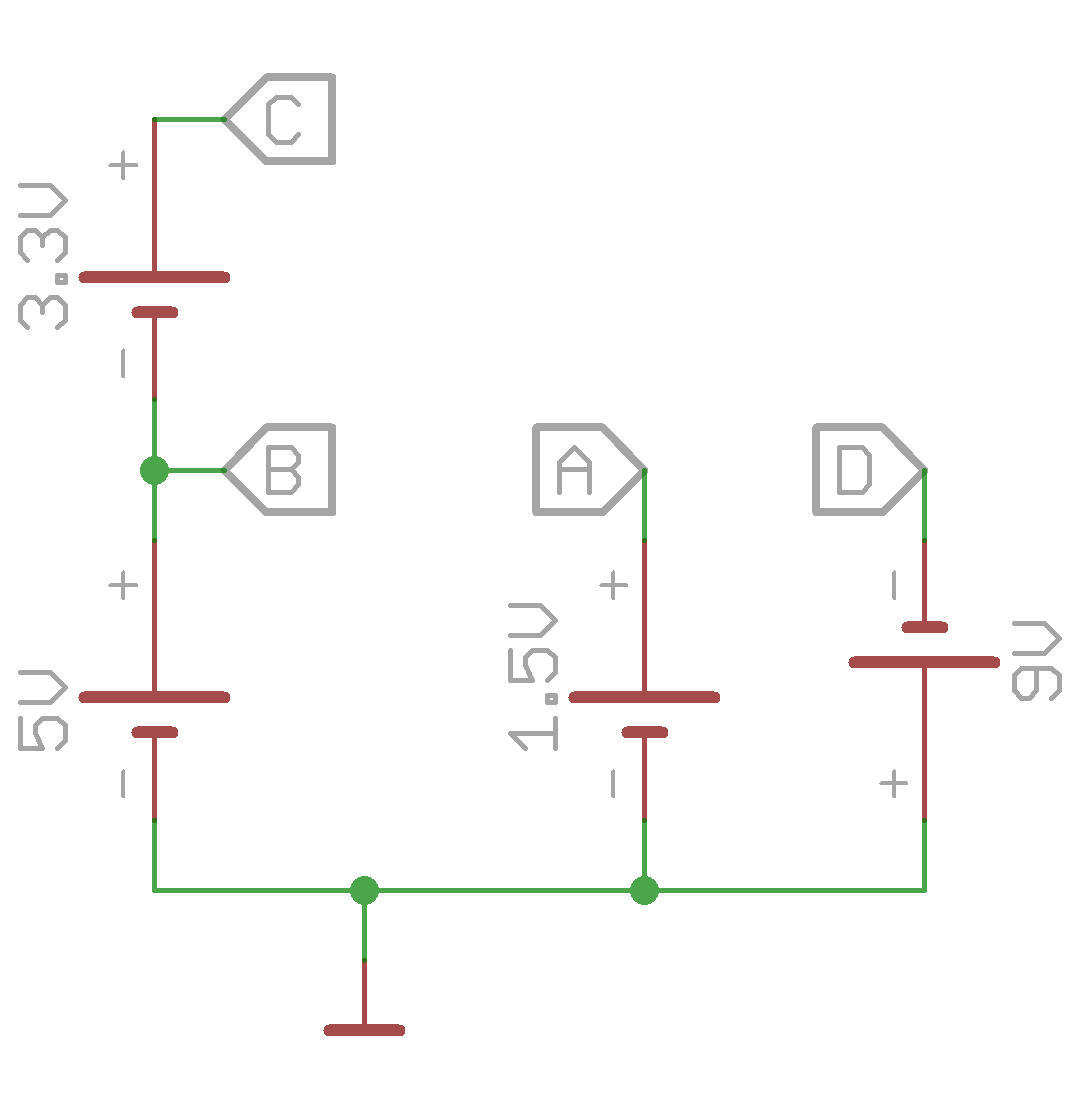
\includegraphics[width=.5\textwidth,height=.75\textheight,keepaspectratio]{e02/Spannung.png}
      \caption{Spannungsquellen in einem Netzwerk mit möglichen Messpunkten}
    \end{figure}
  \end{center}
\end{frame}

\begin{frame}
  \frametitle{Digitales Multimeter}
  \begin{center}
    \begin{figure}
      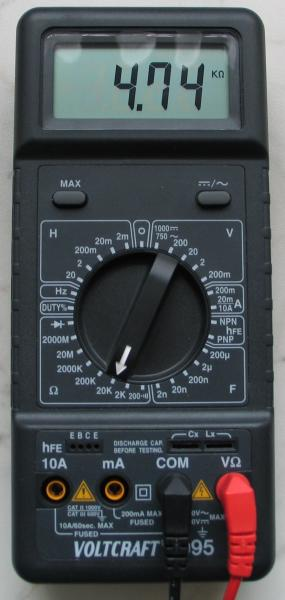
\includegraphics[width=.25\textwidth,height=.75\textheight,keepaspectratio]{e02/digitalmultimeter.jpg}
      \attribcaption{Digitales Multimeter}{MichaelHaeckel}{https://commons.wikimedia.org/wiki/File:Digitalmultimeter.jpg}{\ccpd}
    \end{figure}
  \end{center}
\end{frame}

\begin{frame}
  \frametitle{Was wo anschließen?}
  \begin{minipage}{0.4\textwidth}
    \begin{figure}
      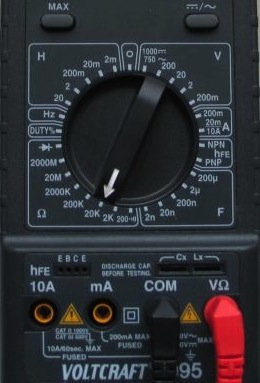
\includegraphics[width=1\textwidth,height=.75\textheight,keepaspectratio]{e02/digitalmultimeterMess.jpg}
      \attribcaption{Digitales Multimeter}{MichaelHaeckel (modifiziert)}{https://commons.wikimedia.org/wiki/File:Digitalmultimeter.jpg}{\ccpd}
    \end{figure}
  \end{minipage}
  \begin{minipage}{0.4\textwidth}
    \begin{itemize}
      \item Was kann alles gemessen werden?
      \item Wo zum Strom messen anschließen?
      \item Wo zum Spannung messen anschließen?
      \item Welcher Messbereich?
    \end{itemize}
  \end{minipage}
\end{frame}

\begin{frame}
  \frametitle{Spannung bestimmen}
  \begin{center}
    \begin{figure}
      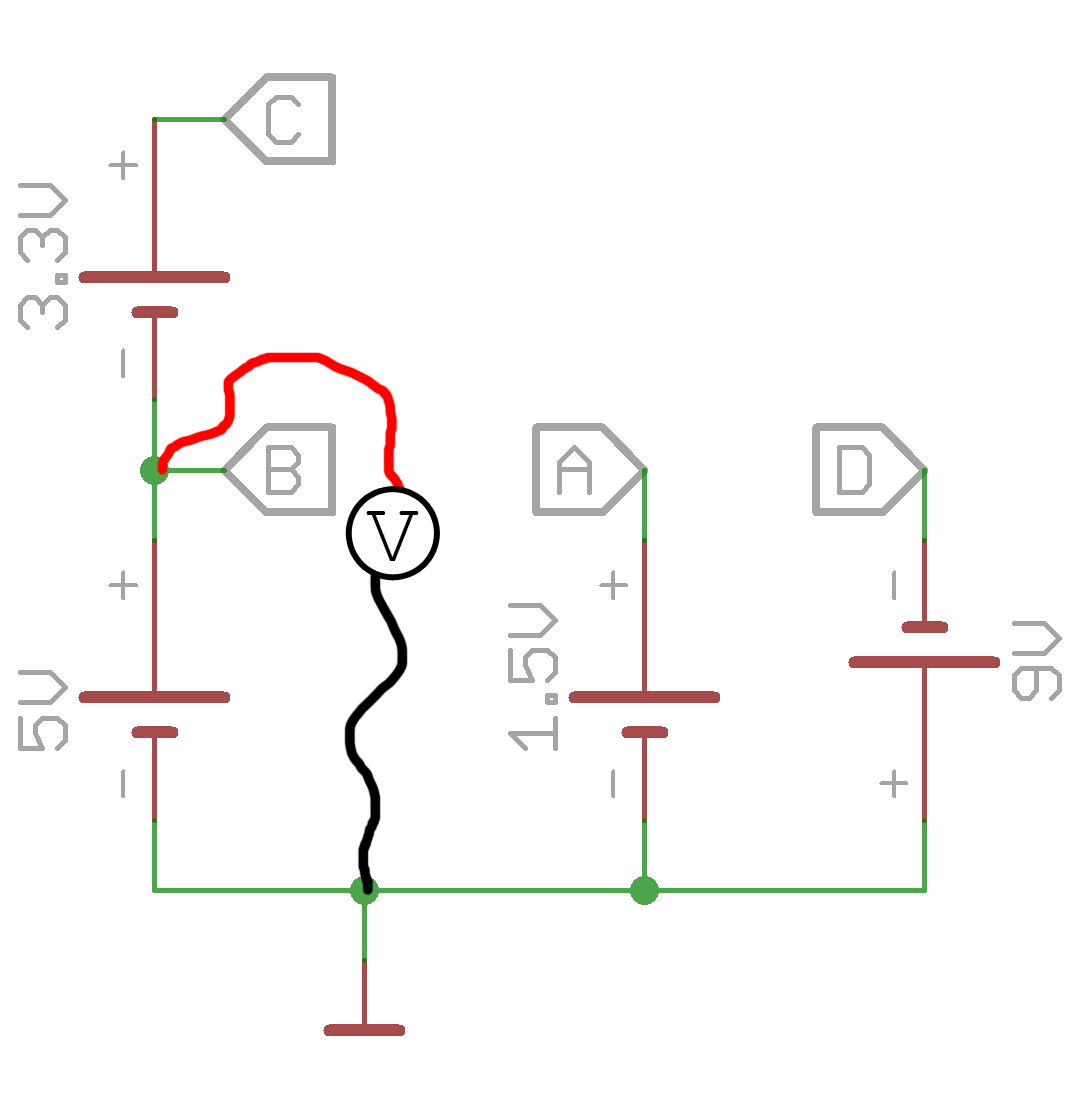
\includegraphics[width=.4\textwidth,height=.75\textheight,keepaspectratio]{e02/SpannungMess.png}
      \caption{Zusatzfrage: Welchen Betrag zeigt das Messgerät beim Messen von $A$ nach $C$ an?}
    \end{figure}
  \end{center}
\end{frame}

\begin{frame}
  \frametitle{Potential}
  \begin{block}{}
    Spannung ist der Potentialunterschied an zwei Punkten.
  \end{block}
  \begin{block}{}
    Ein Multimeter misst den Potentialunterschied.
  \end{block}
  \begin{block}{}
    Nullpotential ist ein theoretisches Modell.
  \end{block}
\end{frame}

\section*{Strom}

\begin{frame}
  \frametitle{Strom}
  \begin{center}
    \begin{block}{}
      Elektrischer Strom ist die gerichtete Bewegung von Ladungsträgern.
    \end{block}
    \begin{block}{}
      Elektrischer Strom $I$ wird in [$A$] Ampere angegeben
    \end{block}
  \end{center}
\end{frame}

\begin{frame}
  \frametitle{Physikalische vs. Technische Stromrichtung}
  \begin{center}
    \begin{figure}
      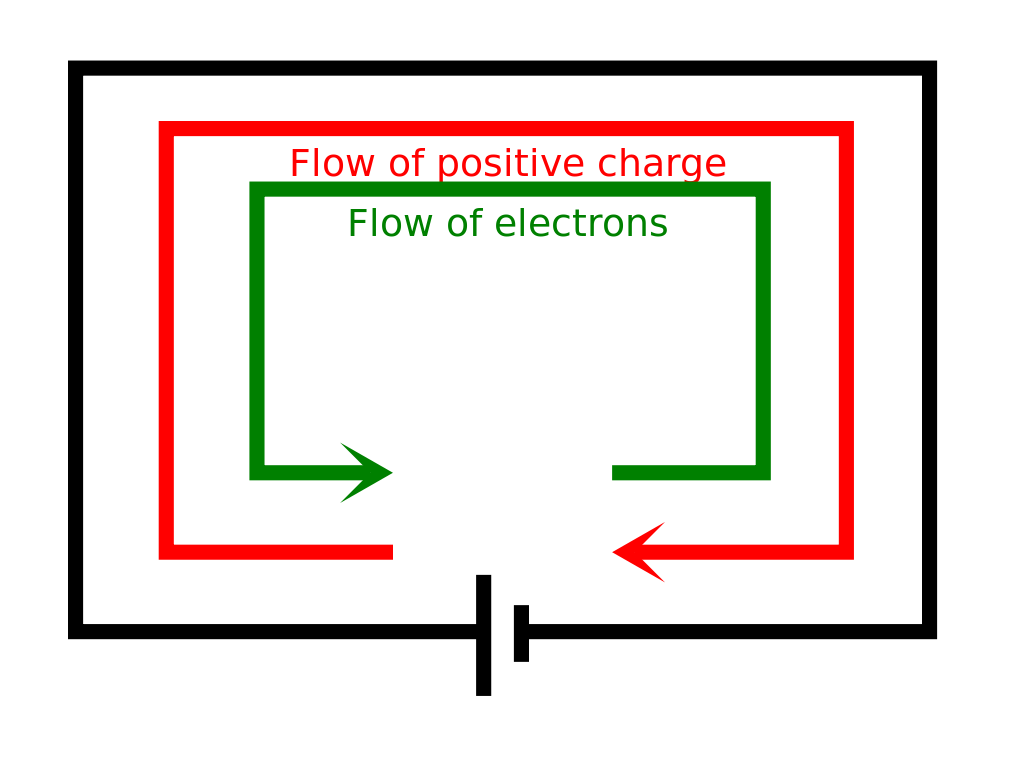
\includegraphics[width=.7\textwidth,height=.75\textheight,keepaspectratio]{e02/Current_notation.png}
      \attribcaption{Nur Elektronen können sich bewegen}{User:Flekstro (Conventional\_Current.png by User:Romtobbi)}{https://commons.wikimedia.org/wiki/File:Current_notation.svg}{\ccby}
    \end{figure}
  \end{center}
\end{frame}

\begin{frame}
  \frametitle{Strom Messen}
  \begin{center}
    \begin{figure}
      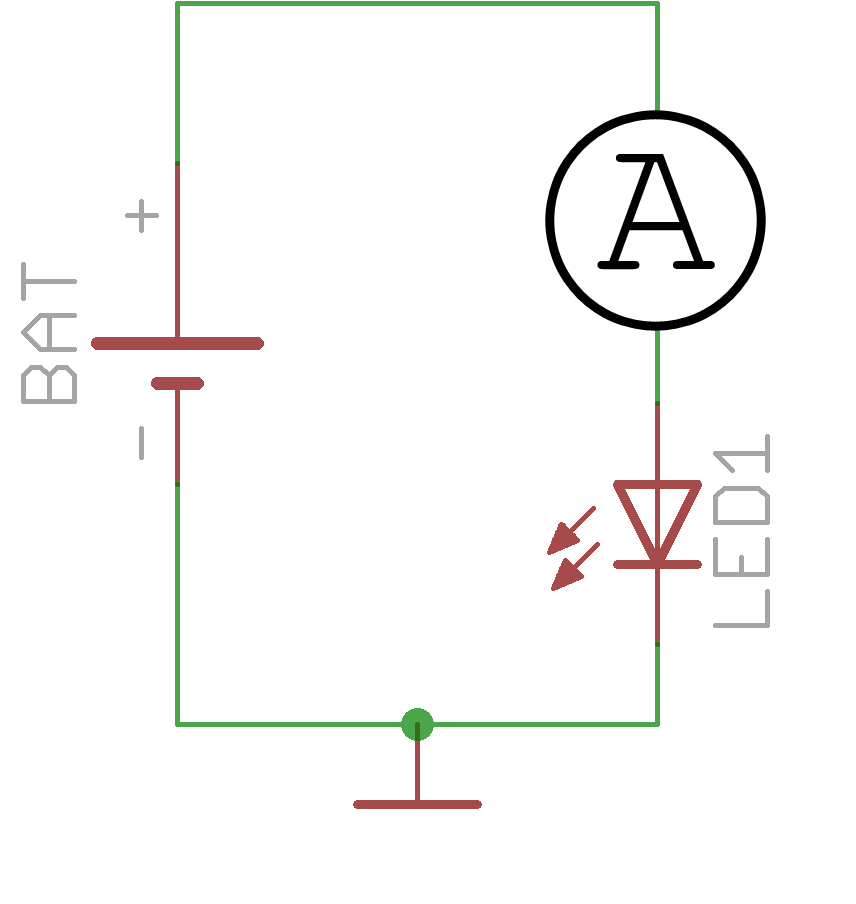
\includegraphics[width=.5\textwidth,height=.75\textheight,keepaspectratio]{e02/reiheAmpare.png}
      \caption{Strom wird in Reihe gemessen}
    \end{figure}
  \end{center}
\end{frame}

\begin{frame}
  \frametitle{Wie sollte gemessen werden?}
  \begin{figure}
    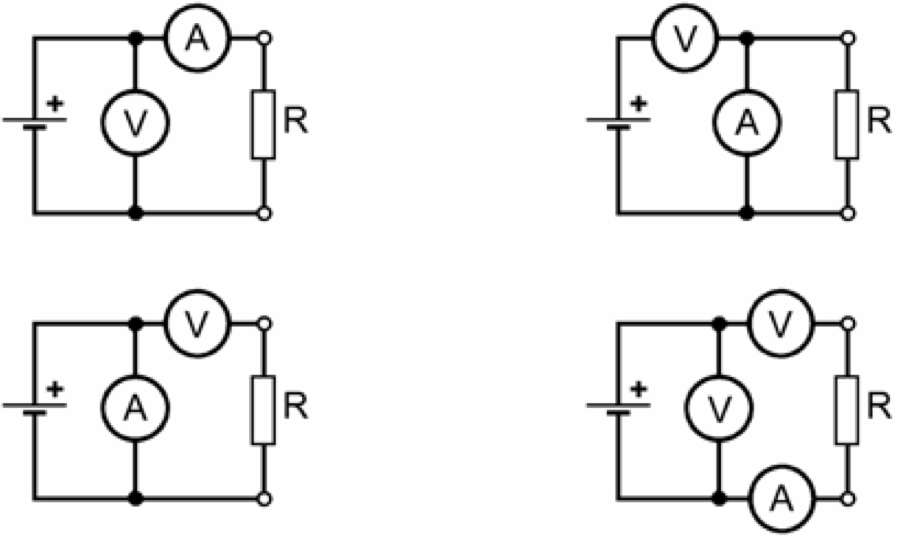
\includegraphics[width=\textwidth,height=.75\textheight,keepaspectratio]{e02/stromSpannung.png}
    \caption{Fragenkatalog Bundesnetzagentur Klasse E TJ201}
  \end{figure}
\end{frame}

\section*{Ladung}

\begin{frame}
  \frametitle{Ladung}
  \begin{center}
    \begin{figure}
      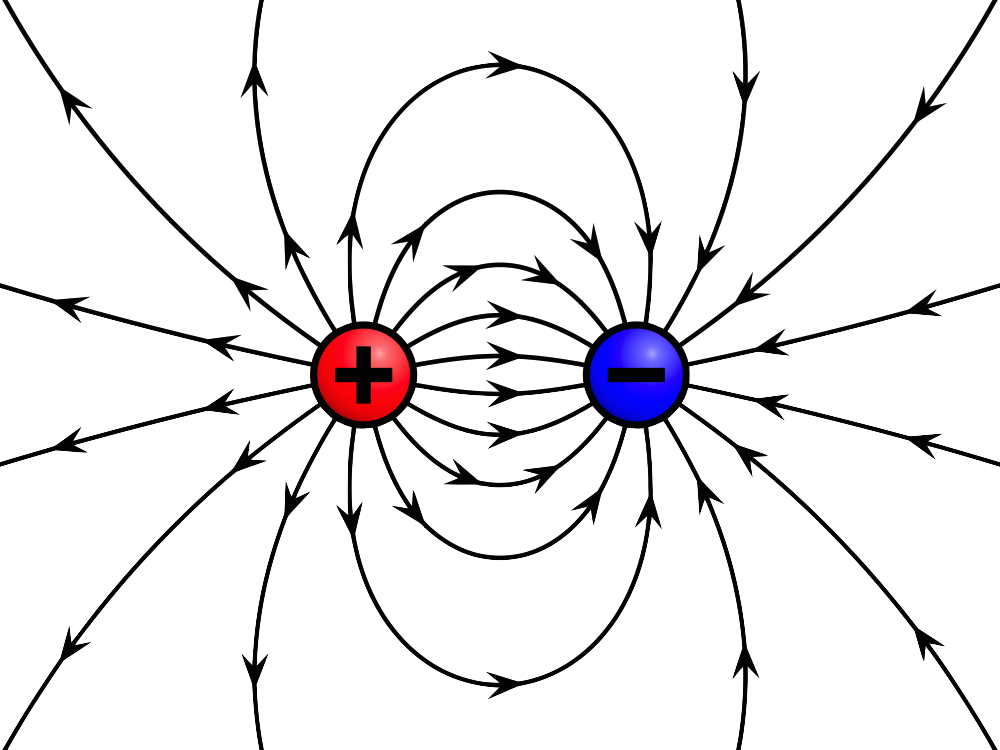
\includegraphics[width=\textwidth,height=.75\textheight,keepaspectratio]{e02/ladung.png}
      \attribcaption{$Q = I \cdot t$}{Geek3}{https://commons.wikimedia.org/wiki/File:VFPt_charges_plus_minus_thumb.svg}{\ccbysa}
    \end{figure}
  \end{center}
\end{frame}

\begin{frame}
  \frametitle{Prüfungsfrage}
  \begin{tabular}{l||p{.8\textwidth}}\hline
    \textbf{TB205} & \textbf{Wie lange könnte man mit einem voll geladenen Akku mit 55\,Ah einen Amateurfunk-Empfänger betreiben, der einen Strom von 0,8\,Ampere aufnimmt?} \\ \hline\hline
    A & 68 Stunden und 75\,Minuten \\ \hline
    B & Genau 44\,Stunden \\ \hline
    C & 6 Stunden 52\,min und 30\,s \\\hline
    D \only<2>\checkmark & 68\,Stunden und 45\,Minuten \\\hline
  \end{tabular}
  \pause
  \begin{align}
    t = \frac{Q}{I} = \frac{55 Ah}{0,8 A} = 68,75 h = 68 h 45 min
  \end{align}
\end{frame}


\section*{Wechsel\-spannung}

\begin{frame}
  \frametitle{Wechselspannungen}
  \begin{minipage}{0.4\textwidth}
    \begin{figure}
      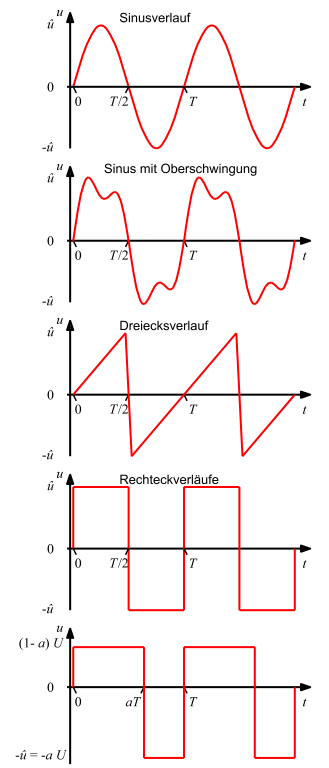
\includegraphics[width=.5\textwidth,height=.75\textheight,keepaspectratio]{e02/Wechselspannungsformen.png}
      \attribcaption{Wechselspannungsformen}{Saure}{https://commons.wikimedia.org/wiki/File:Wechselspannungsformen.svg}{\ccbysa}
    \end{figure}
  \end{minipage}
  \begin{minipage}{0.4\textwidth}
    \begin{itemize}
      \item Verschiedene Formen von Wechselspannung
      \item Beim Morsen bestenfalls ein Sinus
      \item Ganz verschiedene Frequenzen
      \item Stromnetz im Hause: $50Hz$
      \item $70cm$ AFu Band $435.000.000Hz$
    \end{itemize}
  \end{minipage}
\end{frame}

\begin{frame}
  \frametitle{Effektivwert vs Spitzen Wert}
  \begin{align}
    \int \! sin^2(\omega t) \, \mathrm{d}t & = \frac{t}{2} - \frac{1}{4\omega}sin^2(2\omega t) + c \\
    U_{eff}^2 \cdot \int_0^T \! sin^2(\omega t) \, \mathrm{d}t & = \frac{T}{2} \cdot \frac{u_{spitze}^2}{T} \\
    U_{eff} & = \frac{1}{\sqrt{2}} u_{spitze}
  \end{align}
  \begin{center}
    \begin{figure}
      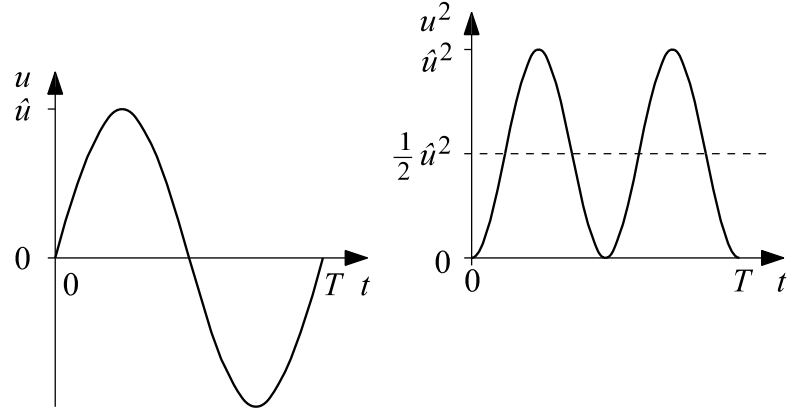
\includegraphics[width=.6\textwidth,height=.3\textheight,keepaspectratio]{e02/EffektivwertSinus.png}\\
      \attribcaption{Effektivwert-Sinus}{Saure}{https://de.wikipedia.org/wiki/Datei:Effektivwert-Sinus.svg}{\ccbysa}
    \end{figure}
  \end{center}
\end{frame}

\begin{frame}
  \frametitle{Effektivwert vs. Spitzenwert}
  \begin{align}
    U_{eff} & = \frac{1}{\sqrt{2}} u_{spitze}
  \end{align}
  \begin{alertblock}{Hausaufgabe}
    Aufgabe: Berechne den Spitzenwert des ``Hausstroms'' mit $U_{eff} = 240V$
  \end{alertblock}
\end{frame}

\section*{Referenzen}

\begin{frame}
  \frametitle{Referenzen/Links}

  \footnotesize
  \begin{itemize}
    \item Moltrecht E 02: \\
      \url{https://www.darc.de/der-club/referate/ajw/lehrgang-te/e02/}
  \end{itemize}

\end{frame}

% Hier könnte noch eine Kontaktfolie stehen

\end{document}

